%%%
%
% $Autor: Wings $
% $Datum: 2021-05-14 $
% $Pfad: GitLab/MLEdgeComputer $
% $Dateiname: 
% $Version: 4620 $
%
% !TeX spellcheck = de_DE/GB
% !TeX program = pdflatex
% !BIB program = biber/bibtex
% !TeX encoding = utf8
%
%%%



\chapter{Portable Document Format (PDF)}

\section{Portable Document Format (PDF)}, Introduced by Adobe, the PDF (Portable Document Format) is a highly versatile file format known for its robustness and accessibility in presenting and exchanging documents, regardless of the software, hardware, or operating systems used by end-users. Now an open standard maintained by the International Organization for Standardization (ISO), the PDF format boasts extensive capabilities\cite{Adobe:2025}.

 PDF documents can include a range of interactive elements such as hyperlinks, buttons, form fields, and multimedia content like audio and video files. Additionally, PDFs support electronic signatures, offering a secure and verifiable method for digital document authentication. The format's compatibility across both Windows and macOS platforms, aided by the freely available Adobe Acrobat Reader, further enhances its universal accessibility.


The genesis of the PDF format can be traced back to 1991, when Adobe co-founder Dr. John Warnock initiated the Camelot Project. This project aimed to revolutionize the transition from paper-based to digital documentation by enabling the capture and electronic transmission of documents from any application. By 1992, this initiative had evolved into the Portable Document Format (PDF), which is now extensively utilized by businesses worldwide.

 Adobe software generates PDFs that preserve the original document formatting, ensuring accurate reproduction of text, graphics, and spreadsheets. These PDFs comply with ISO 32000 standards for electronic document exchange and include various specialized standards, such as PDF/A for long-term archiving, PDF/E for engineering documentation, and PDF/X for prepress graphics exchange. Additionally, the format adheres to accessibility standards, enhancing usability for individuals with disabilities.

\begin{itemize}
  \item Adobe offers user-friendly tools for managing PDFs, such as the Adobe Acrobat Reader mobile application and the Acrobat Sign mobile application, which facilitate the use of electronic signatures. PDFs can be accessed through any web browser or operating system. For executing legally binding signatures, it is recommended to use Adobe Acrobat or Acrobat Sign.

  \item Security features are integral to the PDF format, enabling users to apply password protection, redact sensitive information, and detect and remove hidden data. Adobe collaborates with major corporations to integrate Adobe Document Cloud’s PDF tools into existing software ecosystems, such as Microsoft 365. This integration streamlines workflows by allowing instant conversion of Microsoft Word, Excel, or PowerPoint files into PDF format. Additionally, Adobe tools support the creation of PDFs from scanned paper documents using optical character recognition (OCR) technology. Adobe Acrobat Pro goes beyond basic PDF viewing, offering a comprehensive suite of tools for creating, editing, and converting PDF files to various formats, thereby ensuring a seamless and efficient document management experience.

\end{itemize}


\section{Types of PDFs}

Understanding the specific type of PDF file is crucial when working with PDFs. While the conventional PDF format is widely used for storing and sharing documents online, there are various types of PDFs, each serving distinct functions.//

These formats can be categorized into two groups: those adhering to International Organization for Standardization (ISO) standards and those modified to meet the requirements of other organizations. Let's explore the different PDF types and their typical applications.

There are nine distinct PDF types:
\begin{enumerate}
\item PDF:This is considered the standard PDF format, widely used for file sharing and viewing online.

\item PDF/A: This type of PDF is favored by managers and archivists for long-term file storage. It features a restricted set of capabilities, excluding elements like JavaScript, audio, and video content, to ensure longevity and stability.

\item PDF/E: Tailored to support construction, engineering, and manufacturing specifications, this PDF format is prevalent in those industries.

\item PDF/X: Graphic designers and print professionals commonly use this PDF type, which is specifically designed to enhance graphic support during sharing and printing processes.

\item PDF/VT: Similar to PDF/X but offering additional customization features, this file type is well-suited for print professionals and graphic designers who require more flexibility and control over their documents.

\item PDF/UA: Designed to be compatible with assistive technology, this PDF format enhances readability and navigation for individuals with disabilities.

\item PAdES: This format establishes standards for PDF Advanced Electronic Signatures, ensuring compliance with major legislation.

\item PDF Healthcare: This format was developed to ensure best practices for handling and managing healthcare information.

\item Searchable PDF: Essentially a standard PDF file with a search function, this type makes image-based PDFs text-searchable through the use of optical character recognition (OCR) technology.
\end{enumerate}

Seven of these formats adhere to ISO standards:
\begin{enumerate}
\item PDF
\item PDF/A
\item PDF/E
\item PDF/X
\item PDF/VT
\item PDF/UA
\item Searchable PDF
\end{enumerate}
Meanwhile, two have been adapted by additional organizations to suit their specific needs:
\begin{enumerate}
\item PAdES
\item PDF Healthcare.
\end{enumerate}
\cite{Lozano:2024}

\bigskip

\section{What are PDF file types used for?}

PDFs boast a multitude of capabilities, and to fully understand these, it is essential to familiarize yourself with the specific PDF file type you are working with. Generally, however, the suite of PDF-based extensions serves the following purposes:

\begin{itemize}
\item Preserving document formatting:PDFs, as a portable document format, are instrumental in retaining crucial information within the file, including text formatting, images, hyperlinks, and comments.

\item Effortlessly sharing and viewing files:The standard PDF format seamlessly aligns with most computers and devices, making it easy to open and share files across the web without compatibility concerns.

\item Securing confidential documents:PDF documents provide a mechanism to safeguard sensitive information by allowing users to secure files with passwords and impose restrictions on specific features such as viewing or editing.

\item Streamlining electronic signatures:PDF documents enable prompt signing, sending, and receiving of electronic signatures, eliminating the need for traditional printing methods.
\end{itemize}

\bigskip
\cite{AdobePDF:2024a}.

\section{Advantages of Different Types of PDFs}

When working with or accessing various types of PDFs, numerous advantages can be leveraged:

\begin{itemize}
\item Universally compatible: Standard PDF files can be opened and viewed on most devices, ensuring seamless accessibility.

\item Accessible to a wider audience:An accessible PDF document (PDF/UA) can be read and accessed by individuals with disabilities, such as those who are visually impaired or rely on assistive technologies.

\item Suited for specialist uses: Specific PDF file formats cater to specialized industries, such as PDF/A for archiving, PDF/E for engineering, and PDF/X for printing.

\item Space-efficient storage: PDF files are compressed, resulting in smaller file sizes compared to other formats, making them an attractive option for conserving hard-drive space.

\item Great for sharing and collaborating: Due to their typically smaller size, PDF files can be easily shared via email or uploaded online, facilitating better collaborative efforts.

\item Ease of creation and editing: PDF files are straightforward to create using Adobe Acrobat. Additionally, converting other document formats, such as .DOCX or .DOC, to a PDF file is quick and simple with the Adobe Acrobat online convert to PDF tool.
\end{itemize}

\cite{ABBYY:2023}

\bigskip


%Reference:Adobe. (n.d.). About Adobe PDF. Retrieved from https://www.adobe.com/acrobat/about-adobe-pdf.html
\newpage
\section{Python Packages for PDF Handling}

PDF handling, particularly concerning text, image, and table extraction, refers to the process of programmatically extracting meaningful information from PDF (Portable Document Format) files. PDFs are commonly used for document distribution, and they can contain various elements such as text, images, and tables, which we will need for our project. Extracting these elements programmatically is crucial for various applications, including data analysis, content parsing, and document processing. Here's what each aspect entails:
\begin{itemize}
\item Text Extraction: Text extraction involves extracting textual content from PDF files. Extracting text allows for content analysis, searching, and repurposing of information contained in PDF documents.

\item Image Extraction: Image extraction involves extracting images embedded within PDF files. Extracting images is crucial for tasks involving visual content, such as image recognition, content understanding, and multimedia processing.

\item Table Extraction: Table extraction involves identifying and extracting tabular data present in PDF files. Extracting tables is essential for converting tabular data into a structured format suitable for analysis and further processing.
\end{itemize}

\newpage

\usetikzlibrary{shapes.geometric, arrows}

\tikzstyle{startstop} = [rectangle, rounded corners, minimum width=2cm, minimum height=1cm, text centered, draw=black, fill=black!30]
\tikzstyle{process} = [rectangle, minimum width=2cm, minimum height=1cm, text centered, draw=black, fill=blue!30]
\tikzstyle{decision} = [diamond, aspect=1.5, minimum width=1.5cm, minimum height=1cm, text centered, draw=red, fill=red!10]
\tikzstyle{arrow} = [thick,->,>=stealth]


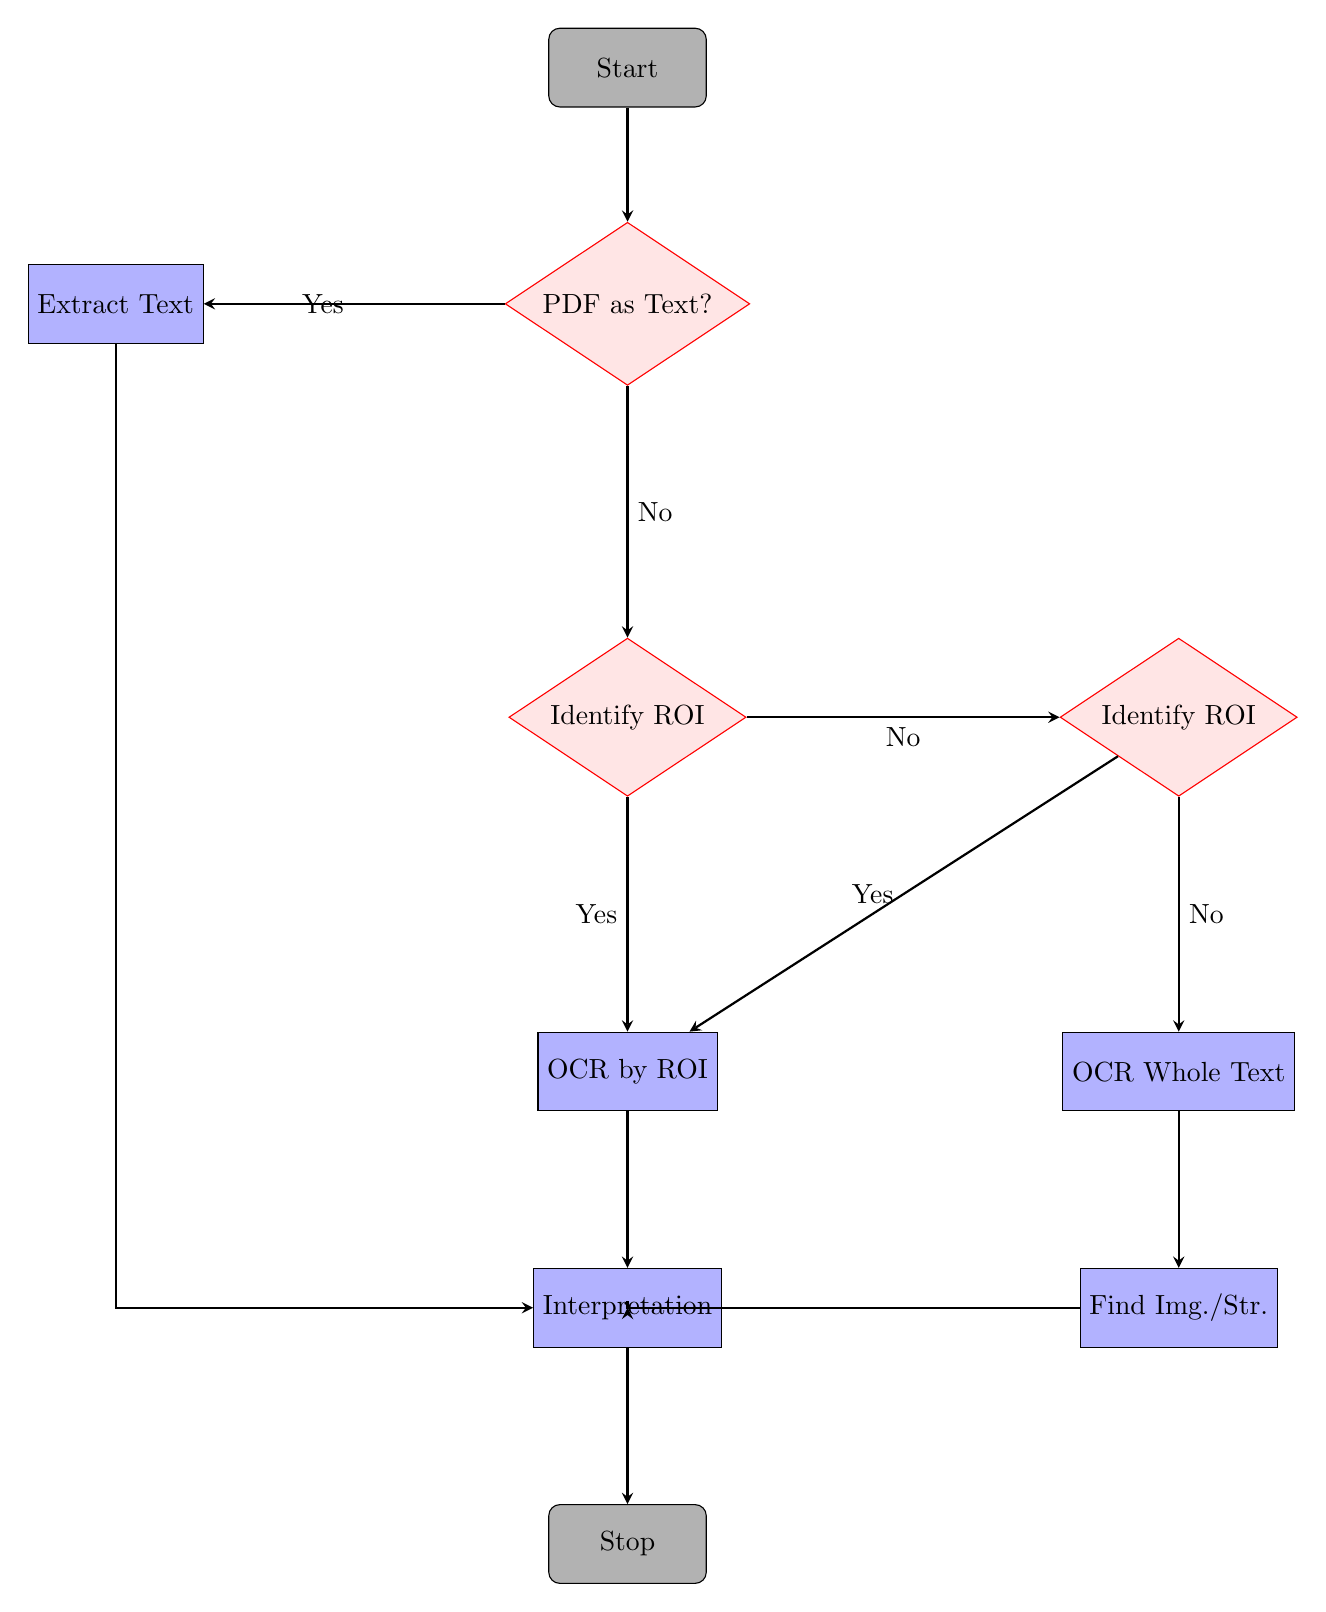
\begin{tikzpicture}[node distance=3 cm]
    % Nodes
    \node (start) [startstop] {Start};
    \node (dec1) [decision, below of=start] {PDF  as  Text?};
    \node (pro1) [process, left of=dec1, xshift=-3.5cm] {Extract Text};
    \node (dec2) [decision, below of=dec1, yshift=-2.25cm] {Identify ROI};
    \node (dec3) [decision, right of=dec2, xshift=4cm] {Identify ROI};
    \node (pro2) [process, below of=dec2, yshift=-1.5cm] {OCR by ROI};
    \node (pro3) [process, below of=dec3, yshift=-1.5cm] {OCR Whole Text};
    \node (pro4) [process, below of=pro3] {Find Img./Str.};
    \node (pro5) [process, below of=pro2] {Interpretation};
    \node (stop) [startstop, below of=pro5] {Stop};

    % Arrows
    \draw [arrow] (start) -- (dec1);
    \draw [arrow] (dec1) -- node[anchor=east] {Yes} (pro1);
    \draw [arrow] (dec1) -- node[anchor=west] {No} (dec2);
    \draw [arrow] (dec2) -- node[anchor=east] {Yes} (pro2);
    \draw [arrow] (dec2) -- node[anchor=north] {No} (dec3);
    \draw [arrow] (dec3) -- node[anchor=east] {Yes} (pro2);
    \draw [arrow] (dec3) -- node[anchor=west] {No} (pro3);
    \draw [arrow] (pro1) |- (pro5);
    \draw [arrow] (pro2) -- (pro5);
    \draw [arrow] (pro3) -- (pro4);
    \draw [arrow] (pro4) -| (pro5);
    \draw [arrow] (pro5) -- (stop);
\end{tikzpicture}






Handling PDFs in Python involves using various libraries and tools that provide functionalities for reading, manipulating, and extracting content from PDF files. Here are some popular Python libraries and tools for handling PDFs:

\begin{enumerate}
\item PyPDF2: Allows basic PDF operations like merging, splitting, and extracting text.
%GitHub Repository: https://github.com/mstamy2/PyPDF2
\item PyTesseract: PyTesseract is a Python wrapper for Google's Tesseract-OCR Engine. It can be used for optical character recognition (OCR) to extract text from images.
\item pdfplumber: Focuses on extracting text, images, and tables from PDFs. Built on top of the PDF parsing library pdfminer.
%GitHub Repository: https://github.com/jsvine/pdfplumber
\item Tabula-py: Primarily designed for extracting tables from PDFs.
%GitHub Repository: https://github.com/chezou/tabula-py
\item PyMuPDF (MuPDF): Provides both basic PDF operations and advanced text extraction functionalities.
%GitHub Repository: https://github.com/pymupdf/PyMuPDF
\item PDFMiner.six: A Python library for extracting text, images, and metadata from PDF files.
%GitHub Repository: https://github.com/pdfminers/pdfminer.six
\item Slate: Primarily focuses on text extraction from PDFs.
%GitHub Repository: https://github.com/timClicks/slate
\item Camelot: Designed for extracting tables from PDFs.
%GitHub Repository: https://github.com/camelot-dev/camelot
\item PyPDFium: A Python library for extracting text, images, and metadata from PDF files.
%GitHub Repository: https://github.com/glyph/Pdfium
\item PDFQuery: Allows querying and analyzing PDF documents in Python.
%GitHub Repository: https://github.com/jcushman/pdfquery
\item PDF.js (JavaScript) (usable in Python with tools like pdf2image or pdf2json): A JavaScript library for rendering PDFs in the browser. Useful for web-based PDF applications.
%GitHub Repository: https://github.com/mozilla/pdf.js
\end{enumerate}

These Python packages cover a range of PDF handling tasks, from basic operations to more specialized tasks like table extraction. 


%%%
\section{Relevance of Packages}

\subsection{Outdated and Underdevelopment}

\textbf{Outdated Packages:}
\begin{enumerate}
\item Slate:
%https://github.com/timClicks/slate
Last Commit: About 7 years ago (as of my last knowledge update in January 2022).
Status: Potentially inactive or incomplete. A lack of recent updates could indicate the project is not actively maintained.
\item PyPDFium:
%https://github.com/PDFium/PDFium
Last Commit: About 5 years ago (as of my last knowledge update in January 2022).
Status: Potentially inactive or incomplete. A lack of recent updates could indicate the project is not actively maintained.
\item PyPDF2: PyPDF2 has been discarded recently.
%https://www.knowledgehut.com/blog/programming/working-with-pdf-files-in-python
\end{enumerate}



\subsection{Output from Packages}



\begin{tabular}{llllllllll}
\hline
\multicolumn{1}{|l|}{\rotatebox{90}{Python PDF Packages}}                      & \multicolumn{1}{l|}{\rotatebox{90}{String/Text}}                & \multicolumn{1}{l|}{\rotatebox{90}{Python DataFrame}} & \multicolumn{1}{l|}{\rotatebox{90}{CSV}} & \multicolumn{1}{l|}{\rotatebox{90}{JSON}} & \multicolumn{1}{l|}{\rotatebox{90}{HTML}} & \multicolumn{1}{l|}{\rotatebox{90}{EXCEL}} & \multicolumn{1}{l|}{\rotatebox{90}{Markdown}} & \multicolumn{1}{l|}{\rotatebox{90}{Sqlite}} & \multicolumn{1}{l|}{\rotatebox{90}{TSV}} \\ \hline
\multicolumn{1}{|l|}{{\color[HTML]{374151} \textbf{PyPDF2}}}            & \multicolumn{1}{l|}{{\color[HTML]{374151} \cmark}} & \multicolumn{1}{l|}{{\color[HTML]{374151} \xmark}}                        & \multicolumn{1}{l|}{{\color[HTML]{374151} \xmark}}           & \multicolumn{1}{l|}{{\color[HTML]{374151} \xmark}}            & \multicolumn{1}{l|}{{\color[HTML]{374151} \xmark}}            & \multicolumn{1}{l|}{{\color[HTML]{374151} \xmark}}             & \multicolumn{1}{l|}{{\color[HTML]{374151} \xmark}}                & \multicolumn{1}{l|}{{\color[HTML]{374151} \xmark}}              & \multicolumn{1}{l|}{{\color[HTML]{374151} \xmark}}           \\ \hline
\multicolumn{1}{|l|}{{\color[HTML]{374151} \textbf{PyTesseract}}}       & \multicolumn{1}{l|}{{\color[HTML]{374151} \cmark}} & \multicolumn{1}{l|}{{\color[HTML]{374151} \xmark}}                        & \multicolumn{1}{l|}{{\color[HTML]{374151} \xmark}}           & \multicolumn{1}{l|}{{\color[HTML]{374151} \xmark}}            & \multicolumn{1}{l|}{{\color[HTML]{374151} \xmark}}            & \multicolumn{1}{l|}{{\color[HTML]{374151} \xmark}}             & \multicolumn{1}{l|}{{\color[HTML]{374151} \xmark}}                & \multicolumn{1}{l|}{{\color[HTML]{374151} \xmark}}              & \multicolumn{1}{l|}{{\color[HTML]{374151} \cmark}}          \\ \hline
\multicolumn{1}{|l|}{{\color[HTML]{374151} \textbf{pdfplumber}}}        & \multicolumn{1}{l|}{{\color[HTML]{374151} \xmark}}  & \multicolumn{1}{l|}{{\color[HTML]{374151} \xmark}}                        & \multicolumn{1}{l|}{{\color[HTML]{374151} \cmark}}          & \multicolumn{1}{l|}{{\color[HTML]{374151} \cmark}}           & \multicolumn{1}{l|}{{\color[HTML]{374151} \xmark}}            & \multicolumn{1}{l|}{{\color[HTML]{374151} \xmark}}             & \multicolumn{1}{l|}{{\color[HTML]{374151} \xmark}}                & \multicolumn{1}{l|}{{\color[HTML]{374151} \xmark}}              & \multicolumn{1}{l|}{{\color[HTML]{374151} \xmark}}           \\ \hline
\multicolumn{1}{|l|}{{\color[HTML]{374151} \textbf{Tabula-py}}}         & \multicolumn{1}{l|}{{\color[HTML]{374151} \cmark}} & \multicolumn{1}{l|}{{\color[HTML]{374151} \cmark}}                       & \multicolumn{1}{l|}{{\color[HTML]{374151} \cmark}}          & \multicolumn{1}{l|}{{\color[HTML]{374151} \cmark}}           & \multicolumn{1}{l|}{{\color[HTML]{374151} \xmark}}            & \multicolumn{1}{l|}{{\color[HTML]{374151} \xmark}}             & \multicolumn{1}{l|}{{\color[HTML]{374151} \xmark}}                & \multicolumn{1}{l|}{{\color[HTML]{374151} \xmark}}              & \multicolumn{1}{l|}{{\color[HTML]{374151} \cmark}}          \\ \hline
\multicolumn{1}{|l|}{{\color[HTML]{374151} \textbf{PyMuPDF   (MuPDF)}}} & \multicolumn{1}{l|}{{\color[HTML]{374151} \cmark}} & \multicolumn{1}{l|}{{\color[HTML]{374151} \xmark}}                        & \multicolumn{1}{l|}{{\color[HTML]{374151} \xmark}}           & \multicolumn{1}{l|}{{\color[HTML]{374151} \xmark}}            & \multicolumn{1}{l|}{{\color[HTML]{374151} \cmark}}           & \multicolumn{1}{l|}{{\color[HTML]{374151} \xmark}}             & \multicolumn{1}{l|}{{\color[HTML]{374151} \xmark}}                & \multicolumn{1}{l|}{{\color[HTML]{374151} \xmark}}              & \multicolumn{1}{l|}{{\color[HTML]{374151} \xmark}}           \\ \hline
\multicolumn{1}{|l|}{{\color[HTML]{374151} \textbf{PDFMiner.six}}}      & \multicolumn{1}{l|}{{\color[HTML]{374151} \cmark}} & \multicolumn{1}{l|}{{\color[HTML]{374151} \xmark}}                        & \multicolumn{1}{l|}{{\color[HTML]{374151} \xmark}}           & \multicolumn{1}{l|}{{\color[HTML]{374151} \xmark}}            & \multicolumn{1}{l|}{{\color[HTML]{374151} \xmark}}            & \multicolumn{1}{l|}{{\color[HTML]{374151} \xmark}}             & \multicolumn{1}{l|}{{\color[HTML]{374151} \xmark}}                & \multicolumn{1}{l|}{{\color[HTML]{374151} \xmark}}              & \multicolumn{1}{l|}{{\color[HTML]{374151} \xmark}}           \\ \hline
\multicolumn{1}{|l|}{{\color[HTML]{374151} \textbf{Slate}}}             & \multicolumn{1}{l|}{{\color[HTML]{374151} \cmark}} & \multicolumn{1}{l|}{{\color[HTML]{374151} \xmark}}                        & \multicolumn{1}{l|}{{\color[HTML]{374151} \xmark}}           & \multicolumn{1}{l|}{{\color[HTML]{374151} \xmark}}            & \multicolumn{1}{l|}{{\color[HTML]{374151} \xmark}}            & \multicolumn{1}{l|}{{\color[HTML]{374151} \xmark}}             & \multicolumn{1}{l|}{{\color[HTML]{374151} \xmark}}                & \multicolumn{1}{l|}{{\color[HTML]{374151} \xmark}}              & \multicolumn{1}{l|}{{\color[HTML]{374151} \xmark}}           \\ \hline
\multicolumn{1}{|l|}{{\color[HTML]{374151} \textbf{Camelot}}}           & \multicolumn{1}{l|}{{\color[HTML]{374151} \cmark}} & \multicolumn{1}{l|}{{\color[HTML]{374151} \cmark}}                       & \multicolumn{1}{l|}{{\color[HTML]{374151} \cmark}}          & \multicolumn{1}{l|}{{\color[HTML]{374151} \cmark}}           & \multicolumn{1}{l|}{{\color[HTML]{374151} \cmark}}           & \multicolumn{1}{l|}{{\color[HTML]{374151} \cmark}}            & \multicolumn{1}{l|}{{\color[HTML]{374151} \cmark}}               & \multicolumn{1}{l|}{{\color[HTML]{374151} \cmark}}             & \multicolumn{1}{l|}{{\color[HTML]{374151} \xmark}}           \\ \hline
\multicolumn{1}{|l|}{{\color[HTML]{374151} \textbf{PyPDFium}}}          & \multicolumn{1}{l|}{{\color[HTML]{374151} \cmark}} & \multicolumn{1}{l|}{{\color[HTML]{374151} \xmark}}                        & \multicolumn{1}{l|}{{\color[HTML]{374151} \xmark}}           & \multicolumn{1}{l|}{{\color[HTML]{374151} \xmark}}            & \multicolumn{1}{l|}{{\color[HTML]{374151} \xmark}}            & \multicolumn{1}{l|}{{\color[HTML]{374151} \xmark}}             & \multicolumn{1}{l|}{{\color[HTML]{374151} \xmark}}                & \multicolumn{1}{l|}{{\color[HTML]{374151} \xmark}}              & \multicolumn{1}{l|}{{\color[HTML]{374151} \xmark}}           \\ \hline
{\color[HTML]{374151} \textbf{}}                                        & {\color[HTML]{374151} }                         & {\color[HTML]{374151} }                                               & {\color[HTML]{374151} }                                  & {\color[HTML]{374151} }                                   & {\color[HTML]{374151} }                                   & {\color[HTML]{374151} }                                    & {\color[HTML]{374151} }                                       & {\color[HTML]{374151} }                                     & {\color[HTML]{374151} }                                  \\
{\color[HTML]{374151} \textbf{}}                                        & {\color[HTML]{374151} }                         & {\color[HTML]{374151} }                                               & {\color[HTML]{374151} }                                  & {\color[HTML]{374151} }                                   & {\color[HTML]{374151} }                                   & {\color[HTML]{374151} }                                    & {\color[HTML]{374151} }                                       & {\color[HTML]{374151} }                                     & {\color[HTML]{374151} }                                  
\end{tabular}
\captionof{table}{Output Formats for Python Handling Package }
\label{tab:my-table}
\section{Package Compatibilty with PDF types}
\begin{tabular}{llllllllll}
\cline{1-4}
\multicolumn{1}{|l|}{\textbf{Python PDF Packages}}                      & \multicolumn{1}{l|}{Machine Generated}          & \multicolumn{1}{l|}{{\color[HTML]{374151} \textbf{Scanned PDF}}} & \multicolumn{1}{l|}{{\color[HTML]{374151} \textbf{OCR-Processed PDF}}} & {\color[HTML]{374151} \textbf{}} & {\color[HTML]{374151} \textbf{}} & {\color[HTML]{374151} \textbf{}} & {\color[HTML]{374151} \textbf{}} & {\color[HTML]{374151} \textbf{}} & {\color[HTML]{374151} \textbf{}} \\ \cline{1-4}
\multicolumn{1}{|l|}{{\color[HTML]{374151} \textbf{PyPDF2}}}            & \multicolumn{1}{l|}{{\color[HTML]{374151} \cmark}} & \multicolumn{1}{l|}{{\color[HTML]{374151} \xmark}}                   & \multicolumn{1}{l|}{{\color[HTML]{374151} \xmark}}                         & {\color[HTML]{374151} }          & {\color[HTML]{374151} }          & {\color[HTML]{374151} }          & {\color[HTML]{374151} }          & {\color[HTML]{374151} }          & {\color[HTML]{374151} }          \\ \cline{1-4}
\multicolumn{1}{|l|}{{\color[HTML]{374151} \textbf{PyTesseract}}}       & \multicolumn{1}{l|}{{\color[HTML]{374151} \cmark}} & \multicolumn{1}{l|}{{\color[HTML]{374151} \cmark}}                  & \multicolumn{1}{l|}{{\color[HTML]{374151} \cmark}}                        & {\color[HTML]{374151} }          & {\color[HTML]{374151} }          & {\color[HTML]{374151} }          & {\color[HTML]{374151} }          & {\color[HTML]{374151} }          & {\color[HTML]{374151} }          \\ \cline{1-4}
\multicolumn{1}{|l|}{{\color[HTML]{374151} \textbf{pdfplumber}}}        & \multicolumn{1}{l|}{{\color[HTML]{374151} \cmark}} & \multicolumn{1}{l|}{{\color[HTML]{374151} \xmark}}                   & \multicolumn{1}{l|}{{\color[HTML]{374151} Limited}}                    & {\color[HTML]{374151} }          & {\color[HTML]{374151} }          & {\color[HTML]{374151} }          & {\color[HTML]{374151} }          & {\color[HTML]{374151} }          & {\color[HTML]{374151} }          \\ \cline{1-4}
\multicolumn{1}{|l|}{{\color[HTML]{374151} \textbf{Tabula-py}}}         & \multicolumn{1}{l|}{{\color[HTML]{374151} \cmark}} & \multicolumn{1}{l|}{{\color[HTML]{374151} Limited}}              & \multicolumn{1}{l|}{{\color[HTML]{374151} Limited}}                    & {\color[HTML]{374151} }          & {\color[HTML]{374151} }          & {\color[HTML]{374151} }          & {\color[HTML]{374151} }          & {\color[HTML]{374151} }          & {\color[HTML]{374151} }          \\ \cline{1-4}
\multicolumn{1}{|l|}{{\color[HTML]{374151} \textbf{PyMuPDF   (MuPDF)}}} & \multicolumn{1}{l|}{{\color[HTML]{374151} \cmark}} & \multicolumn{1}{l|}{{\color[HTML]{374151} \cmark}}                  & \multicolumn{1}{l|}{{\color[HTML]{374151} \cmark}}                        & {\color[HTML]{374151} }          & {\color[HTML]{374151} }          & {\color[HTML]{374151} }          & {\color[HTML]{374151} }          & {\color[HTML]{374151} }          & {\color[HTML]{374151} }          \\ \cline{1-4}
\multicolumn{1}{|l|}{{\color[HTML]{374151} \textbf{PDFMiner.six}}}      & \multicolumn{1}{l|}{{\color[HTML]{374151} \cmark}} & \multicolumn{1}{l|}{{\color[HTML]{374151} \cmark}}                  & \multicolumn{1}{l|}{{\color[HTML]{374151} \cmark}}                        & {\color[HTML]{374151} }          & {\color[HTML]{374151} }          & {\color[HTML]{374151} }          & {\color[HTML]{374151} }          & {\color[HTML]{374151} }          & {\color[HTML]{374151} }          \\ \cline{1-4}
\multicolumn{1}{|l|}{{\color[HTML]{374151} \textbf{Slate}}}             & \multicolumn{1}{l|}{{\color[HTML]{374151} \cmark}} & \multicolumn{1}{l|}{{\color[HTML]{374151} \xmark}}                   & \multicolumn{1}{l|}{{\color[HTML]{374151} Limited}}                    & {\color[HTML]{374151} }          & {\color[HTML]{374151} }          & {\color[HTML]{374151} }          & {\color[HTML]{374151} }          & {\color[HTML]{374151} }          & {\color[HTML]{374151} }          \\ \cline{1-4}
\multicolumn{1}{|l|}{{\color[HTML]{374151} \textbf{Camelot}}}           & \multicolumn{1}{l|}{{\color[HTML]{374151} \cmark}} & \multicolumn{1}{l|}{{\color[HTML]{374151} \xmark}}                   & \multicolumn{1}{l|}{{\color[HTML]{374151} \cmark}}                        & {\color[HTML]{374151} }          & {\color[HTML]{374151} }          & {\color[HTML]{374151} }          & {\color[HTML]{374151} }          & {\color[HTML]{374151} }          & {\color[HTML]{374151} }          \\ \cline{1-4}
\multicolumn{1}{|l|}{{\color[HTML]{374151} \textbf{PyPDFium}}}          & \multicolumn{1}{l|}{{\color[HTML]{374151} \cmark}} & \multicolumn{1}{l|}{{\color[HTML]{374151} \xmark}}                   & \multicolumn{1}{l|}{{\color[HTML]{374151} Limited}}                    & {\color[HTML]{374151} }          & {\color[HTML]{374151} }          & {\color[HTML]{374151} }          & {\color[HTML]{374151} }          & {\color[HTML]{374151} }          & {\color[HTML]{374151} }          \\ \cline{1-4}
{\color[HTML]{374151} \textbf{}}                                        & {\color[HTML]{374151} }                         & {\color[HTML]{374151} }                                          & {\color[HTML]{374151} }                                                & {\color[HTML]{374151} }          & {\color[HTML]{374151} }          & {\color[HTML]{374151} }          & {\color[HTML]{374151} }          & {\color[HTML]{374151} }          & {\color[HTML]{374151} }          \\
{\color[HTML]{374151} \textbf{}}                                        & {\color[HTML]{374151} }                         & {\color[HTML]{374151} }                                          & {\color[HTML]{374151} }                                                & {\color[HTML]{374151} }          & {\color[HTML]{374151} }          & {\color[HTML]{374151} }          & {\color[HTML]{374151} }          & {\color[HTML]{374151} }          & {\color[HTML]{374151} }          \\ \hline
\end{tabular}
\captionof{table}{Python Handling Package Compatibility with PDF Types}
\label{tab:my-table}

%%%%%%%%%%%%%%%%%%%%%%%%%%%%%%%%%%%%%%%%%%%%%%%


